\documentclass[a4paper,12pt,twoside]{article}

%===========PACOTES
\usepackage[body={175mm,240mm}]{geometry}
%\usepackage[portuguese]{babel}
\usepackage{a1}
\usepackage[english]{babel}
\usepackage[latin1]{inputenc} %permite o uso de acentos
%\usepackage[dvips]{color}
\usepackage{amsfonts,amssymb}
%\usepackage{epsfig}
\usepackage{amsmath}
\usepackage{graphicx}
\usepackage{float}

% makeidx
\usepackage{makeidx}
% make index
\makeindex
%\usepackage[pdftex]{graphicx}


\def\mapright#1#2#3{\smash{\mathop{\hbox to
#3{\rightarrowfill}}\limits^{#1}_{#2}}}

\def\mapleft#1#2#3{\smash{\mathop{\hbox to
#3{\leftarrowfill}}\limits^{#1}_{#2}}}

\def\mapright#1#2{\smash{\mathop{\hbox to 0.90cm{\rightarrowfill}}\limits^{#1}_{#2}}}
\def\mapleft#1#2{\smash{\mathop{\hbox to 0.90cm{\leftarrowfill}}\limits^{#1}_{#2}}}

\def\mapleftright#1#2{\smash{\mathop{\hbox to 0.80cm{\leftarrowfill \rightarrowfill}}\limits^{#1}_{#2}}}
\def\ext{\times \! \vrule depth0pt height5pt width0.35pt}

\def\H{\mathcal H}
\def\D{\mathcal D}
\def\B{\mathcal B}
\def\C{\mathbb C}
\def\R{\mathbb R}
\def\S{\mathbb S}
\def\U{\mathcal U}
\def\Z{\mathbb Z}

\title{All the shapes of spaces: a census of small 3-manifolds
\footnote{2010 Mathematics Subject Classification: 
57M25 and 57Q15 (primary), 57M27 and 57M15 (secondary)}} 
\author{S�stenes L. Lins and Lauro D. Lins}

\date{\today}


\begin{document}


\maketitle
\begin{abstract}


In this work we present a complete (no misses, no duplicates) catalogue for closed, 
connected, orientable and
prime 3-manifolds induced by plane graphs with a 
bipartition of its edge set (blinks) up to 9 edges. 
Blinks form a universal encoding for such manifolds. In fact, each such a manifold
is a subtle class of blinks, \cite{lins2013B}. Blinks are in 1-1 correpondence with
{\em blackboard framed links}, \cite {kauffman1991knots, kauffman1994tlr}
We hope that this census becomes as useful for the study of concrete examples of 3-manifolds
as the tables of knots are in the study of knots and links. 

% Along the years we have made an issue
% in our computational work that it must be reproducible and independently checked by other researchers. 
% Our software {\sf BLINK} is available,
% but currently it lacks yet a good documentation and help is welcome to change this. 
% An Wiki open source project is starting.


\end{abstract}


\section{Introduction} 



After presenting some instances of closed 3-manifolds,
P. Alexandroff says in the English translation (1961) of 
his joint work with D. Hilbert \cite{alexandrov1961elementary}, first
published (1932) in German, \cite{alexandroff1932einfachste}:
{\em ``These few examples will suffice. Let it be remarked here that, at present,
in contrast with the two-dimensional case, the problem of enumerating the 
topological types of manifolds of three and more dimensions is in an apparently 
hopeless state. We are not only far removed from the solution, but even from the first step
toward a solution, a plausible conjecture''.}


John Hempel in his book (1976) {\em 3-Manifolds} \cite{hempel1976} writes 
at the opening of Section 15, entitled {Open Problems:}
{\em ``The ultimate goal of the theory would be in providing solutions to:
 {\em The homeomorphism problem}: provide an {\em effective} procedure
 for determining whether two {\em given} 3-manifolds are homeomorphic, together with
 {\em The classification problem}: {\em effectively} generate a list containing
 exactly one 3-manifold from each homeomorphism class.''}

 
\subsection{A complete duplicate free census of 9-small 3-manifolds}
In references \cite{kauffman1994tlr}, \cite{lins2007blink} and \cite{lins1995gca}
we have defined and show how a {\em blink}, that is, a plane graph with
an arbitrary bipartition of its edges (here presented as 
colors black and gray) induces a well
defined closed oriented 3-manifold. Moreover each such a manifold 
is induced by a blink (in fact, by infinite blinks).
An {\em $n$-small} is a closed, connected, orientable and prime
3-manifold is a manifold induced by a blink with at most $n$ edges.
This paper concludes the proof of the following theorem: 
\begin{theorem}[The first 489 closed orientable 3-manifolds]
Let $\mathbb{M}^3$ be an 9-small 3-manifold.
Then $\mathbb{M}^3$ is homeomorphic to exactly one of the 
3-manifolds induced by the 489  blinks below. Morever all of these are pairwise non-homeomorphic.
(However being redundant, we also present the corresponding 
census for the blackboard framed links. These census are
enlarged in the Appendix.)\\
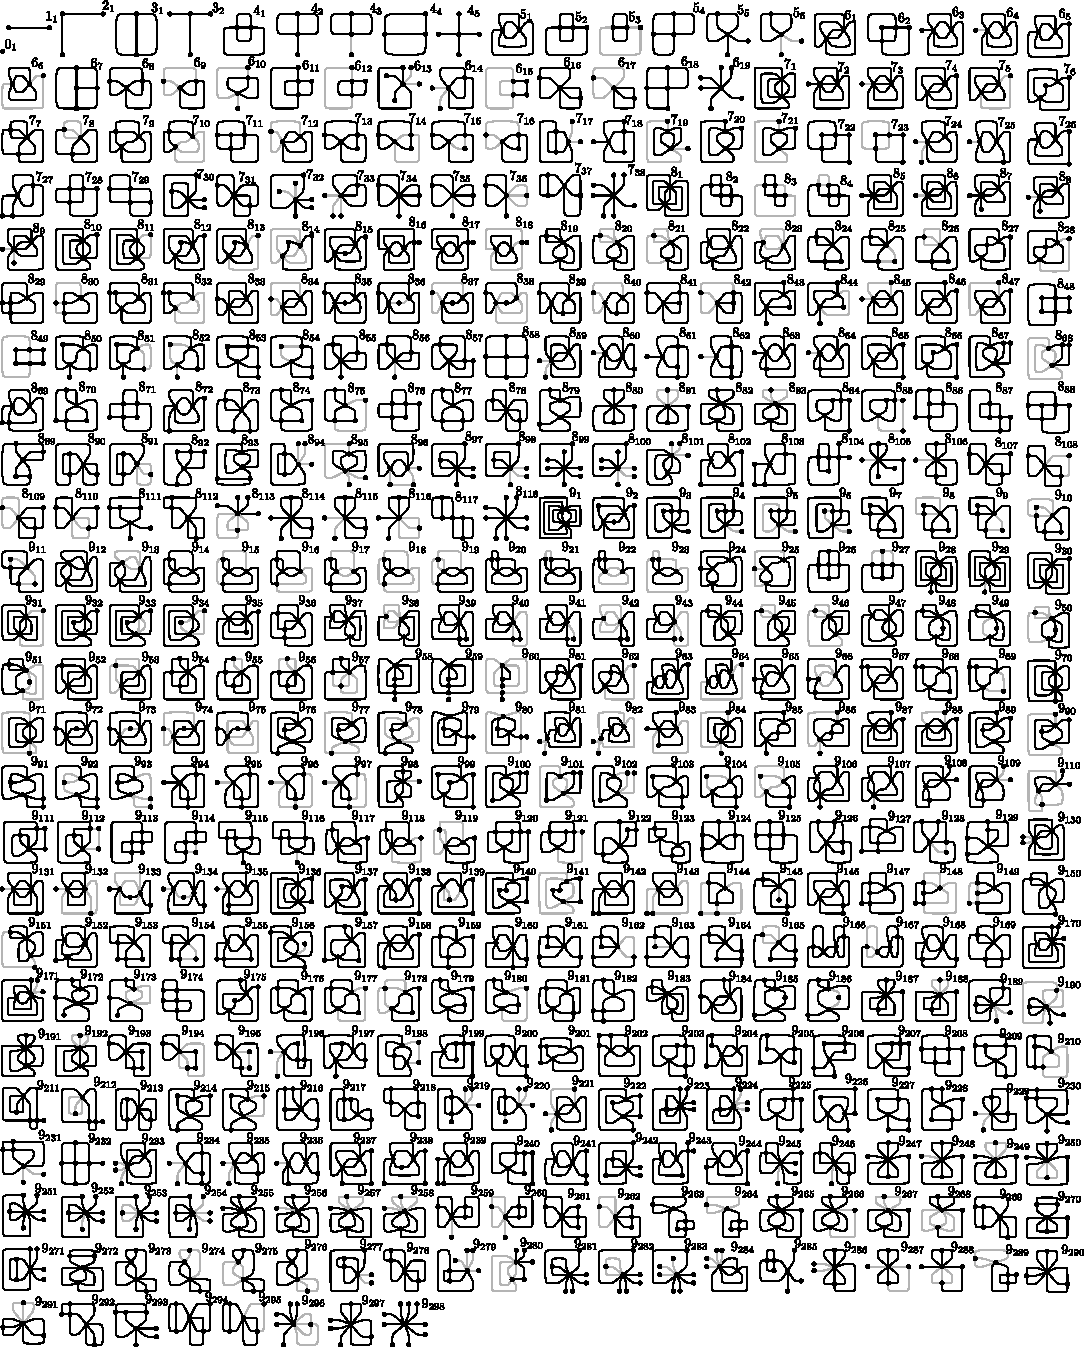
\includegraphics[width=17.5cm]{A.figs/primes489.pdf}\\
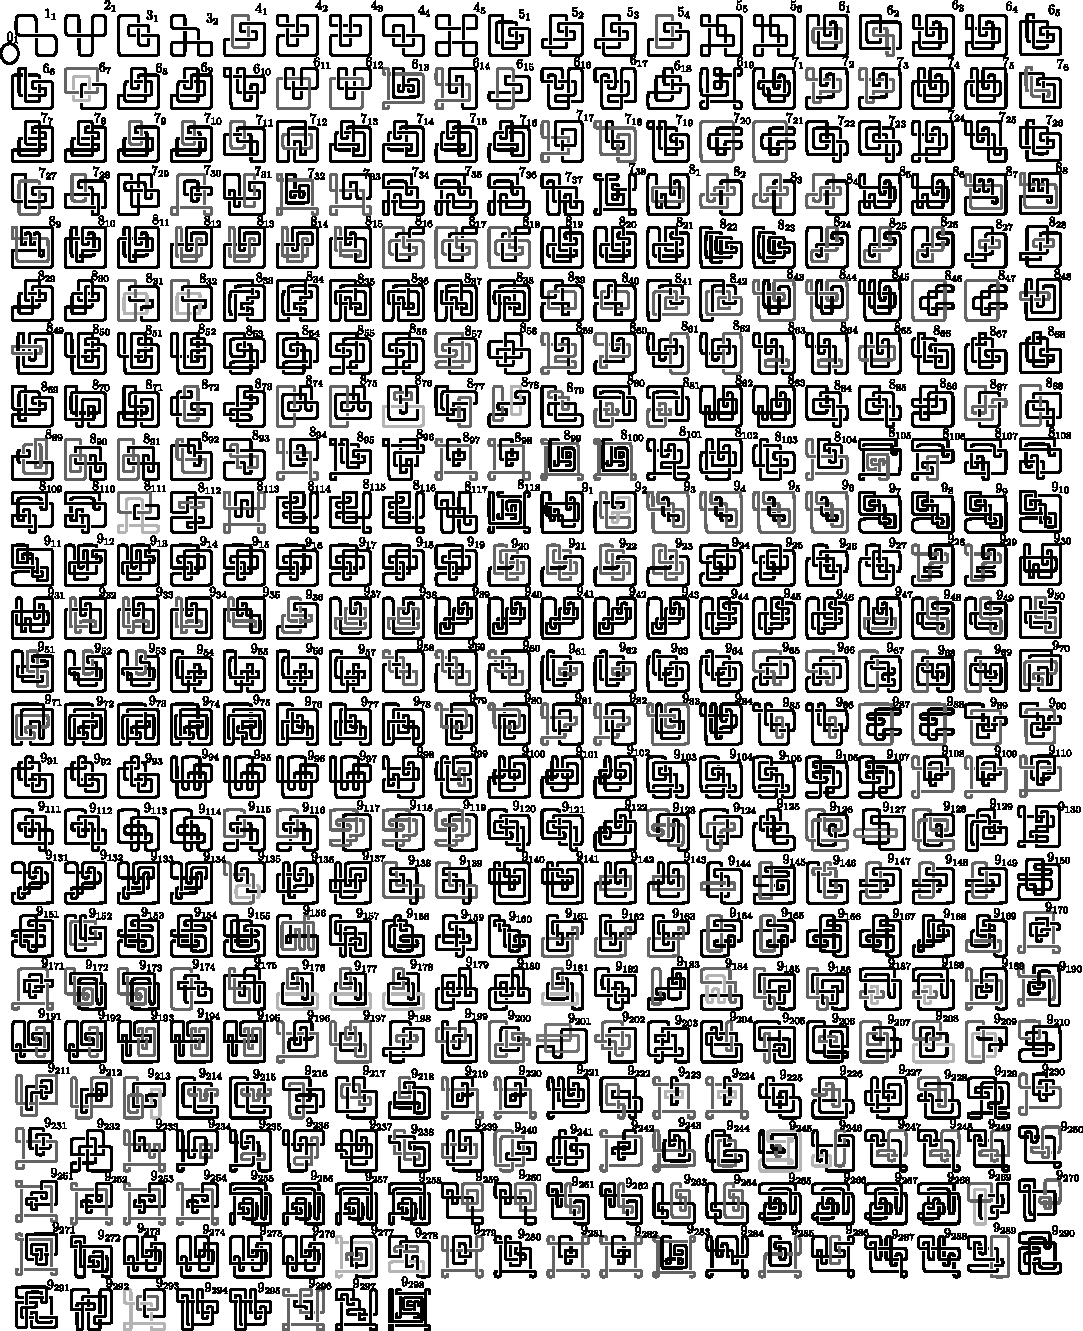
\includegraphics[width=17.5cm]{A.figs/primes489links.pdf} 
\label{theorem:census9}
\end{theorem}

\begin{proof}
 The bulk of the proof follows from L. Lins' thesis under the supervision of S. Lins, 
 \cite{lins2007blink}.
 In this work a theory for blink generation (missing no closed orientable 3-manifolds)
 is provided 
 by pure combinatorics, lexicography and topological filtering of duplicates.
 This resulted in a set $U_9$ with 3437 blinks. This universal set of 9-small 3-manifold
 was partitioned by homology and WRT$_{12}$ (the Witten-Reshetikhin-Turaev invariant 
 computed, as in \cite{kauffman1994tlr} for $r=3,4,\ldots,12)$ into 487 classes, named 
 $HG12QI$-classes. This is achieved by
 explicitly obtaining homeomorphisms between any two blinks in the same $HG12QI$-class.
 Each such homeomorphism is coded into a sequence of gems (defined in the next section)
 that is frozen in the data basis (Mysql) of BLINK forever, and, 
 in principle can be reproduced at will. Exactly 75633 gems were used in the 
 classifing sequences encoding homeomorphisms between the 3-manifolds of $U_9$.
 What remained to be done was to decide the status of the two $HG12QI$-classes
 $9_{126}$ and $9_{199}$ depicted in Fig. \ref{fig:nine126nine199}. After 6 years
 we posted these doubts as a Challenge in the arXiv, \cite{linslins2013A}. 
 In a quick feedback, many Mathematicians got interested in the Challenge (in the order of 
 their comments in the blog)
 \begin{center}
 \begin{verbatim}
 http://ldtopology.wordpress.com/2013/04/23/when-are-two-hyperbolic-
 3-manifolds-homeomorphic/#postcomment.
 \end{verbatim}
 \end{center}
 Comments were by H. Wilton, N. Dunfield, S. Friedl, M. Culler, D. Huberman, J. Berge, 
 C. Doria. Also, N. Dunfield M. Culler and C. Hodgson contacted one of us (S.Lins) via e-mail.
 And we got solutions for the two 6 years old doubts: 
 to the benefit of BLINK both pairs of 3-manifolds are non-homeomorphic.
 M. Culler, N. Dunfield and C. Hodgson sent distinct proofs of this
 fact. Thus there are 489 classes of non-homeomorphic closed 9-small 3-manifolds. More details
 of the distinction are given in Section \ref{sec:resol}.
 \end{proof}
 
 
Relative to page 109 of \cite{lins2007blink} the blinks of 
Theorem \ref{theorem:census9}
have receive two additions, the representative blinks
$U[1563]$ and $U[2165]$. Also the previous HG12QI-class $6_{5}$ became 
the homemorphism class $0_1$
corresponding to $\mathbb{S}^2 \times \mathbb{S}^1$. We have decreased 
by 1 the numbering of the 
$HG12QI$-classes $6_{6}, 6_{7}, \ldots, 6_{20}$ which become the 
homeomorphisms classes  $6_{5}, 6_{7}, \ldots, 6_{19}$:
the HG12QI-classes $9_{126}$ and $9_{199}$ of \cite{lins2007blink} split
into two topological classes. 
We observe that the blinks are enlarged in the appendix, showing them together with the
corresponding blackboard framed links. The notation $n_i$ attached to each blink below,
is the name of its homeomorphism class, not merely its HG12QI-class, as in \cite{lins2007blink}. 

\subsection{Brief historical overview}

 It is amazing how much the picture has changed in the 80 years since the book by 
 Alexandroff and Hilbert.
 The progress initiated with the deep advances in the 1950's and 1960's, starting with
 the proof that 3-manifolds are triangulable by Moise (1952), \cite{moise1952affine}. Next 
 the presentation
 of them by framed links by Lickorish (1962) \cite{lickorish1962representation}.
 Following that Kirby presented its calculus for framed links (1978)\cite{kirby1978calculus}. 
 Starting in the early 1980's W. Thurston's provided gret 
 breakthroughs, developing his conceptual theory 
 on hyperbolic manifolds and of the geometrization conjecture. 
 In the final 1980's early 1990's Witten \cite{witten1989quantum} broke the psicological 
 barrier that there were no good invariants for 3-manifolds. Following that a number of 
 eastern European mathematicians like N. Reshetikhen, V. Turaev and O. Viro, 
 \cite{turaev1992state,reshetikhin1991invariants}
 using quantum groups were able to put in mathematical solid ground Witten's findings.
 One of us, S. Lins, was a witness of the excitement these developments caused. L. H. Kauffman
 and W. B. R. Lickorish discovered the relationship of the Temperley-Lieb algebra with 
 the new invariants,
 \cite{lickorish1991three}. Starting with a sabatical leave in to Chicago in 1990, S. Lins produced
 the joint monography with Kauffman \cite{kauffman1994tlr}, where blinks are first defined 
 and extensive WRT-invariant computations were obtained from the theory developed from scratch,
 independently and simpler than that of quantum groups.  In the early 
 2000's, G. Perelman revolutionized the field proving Poincar�'s Conjecture and
 Thurston's Geometrization Conjecture. More recently in the 2010's, I. Agol is leading the field
 in this era post-Perelman. Of course, this is only a diagonal list of researchers. Many more have contributed and
 some are  extremely active in this era pos-Perelman, \cite{friedl3}. 
 Currently there is a great amount of important reserch issues
 going on and these are exciting times for 3-manifold theory. See the recent essay of E. Klarreich
 in the Simons Foundation, \cite{Klarreich1012}.
         
\section{Blinks and gems}
Unexplored simplicity. This was the reason for birth of this work many years ago.  
Repeating, a {\em blink} is a finite plane graph 
(that is, given embedded in the plane) together with an arbitrary bipartition
of its edges into black and gray. For completeness
we briefly recall the basic definitions of gem theory, leading to its definition, \cite{lins1995gca}
and to its calculus bsed in dipole moves, \cite{ferri1982crystallisation,lins2006blobs}.
A {\em 4-graph} $G$ is a finite bipartite 4-regular graph whose edges are partitioned into 4 colors,
0,1,2, and 3, 
so that at each vertex there is an edge of each color, a proper edge-coloration, \cite{bondy1976gta}.
For each $i \in \{0,1,2,3\}$, let $E_i$ denote the set of $i$-colored edges of $G$.
A $\{j,k\}$-residue in a $4$-graph $G$ is a connected component of the subgraph induced by $E_j \cup E_k$.
A 2-residue is a $\{j,k\}$-residue, for some distinct colors $j$ and $k$.
A {\em gem} is a 4-graph $G$ such that for each color $i$, $G\backslash E_i$ can be embedded in the plane 
such that the boundary of each face is a 2-residue. From a gem there exists a straightforward
algorithm to obtain a closed orientable 3-manifold, in two different, dual ways. 
Every such a manifold is obtainable in this way.
An unecessary big gem is obtained from a triangulation $T$ 
for a manifold by taking the dual of the 
barycentric subdivision of $T$. Here the colors correspond 
to the dimensions. 
Given a pair of vertices $\{u,v\}$ of a gem $G$ with $k$ linking edges $k \in \{0,1,2,3\}$, 
in $k$ distinct colors $K \subset \{0,1,2,3\}$ is called a {\em $K$-dipole} if $u$ and $v$ 
are in distinct $(\{0,1,2,3\})\backslash K$-residues of $G$. A {\em dipole cancellation} is the 
operation that remove $u$, $v$ and their $k$ linking edges leaving $4-k$ pairs of pendant
edges which are reunited along the same colors. The {\em dipole creation} is the inverse move.
The dipole creations and cancellations do not change the induced 3-manifold.
It is possible to simplify substantially the gem corresponding to the dual 
of the barycentric subdivison of a triangulation by cancelling dipoles. 
These simplifications in that gem completely destroys the correspondence of 
colors and dimensions. Two gems induce the same 3-manifold if and only if they are linked 
by a finite sequence of moves where each term is either a dipole cancellation
or a diplole creation, 
\cite{ferri1982crystallisation,lins2006blobs}.

\begin{figure}[!h]
\begin{center}
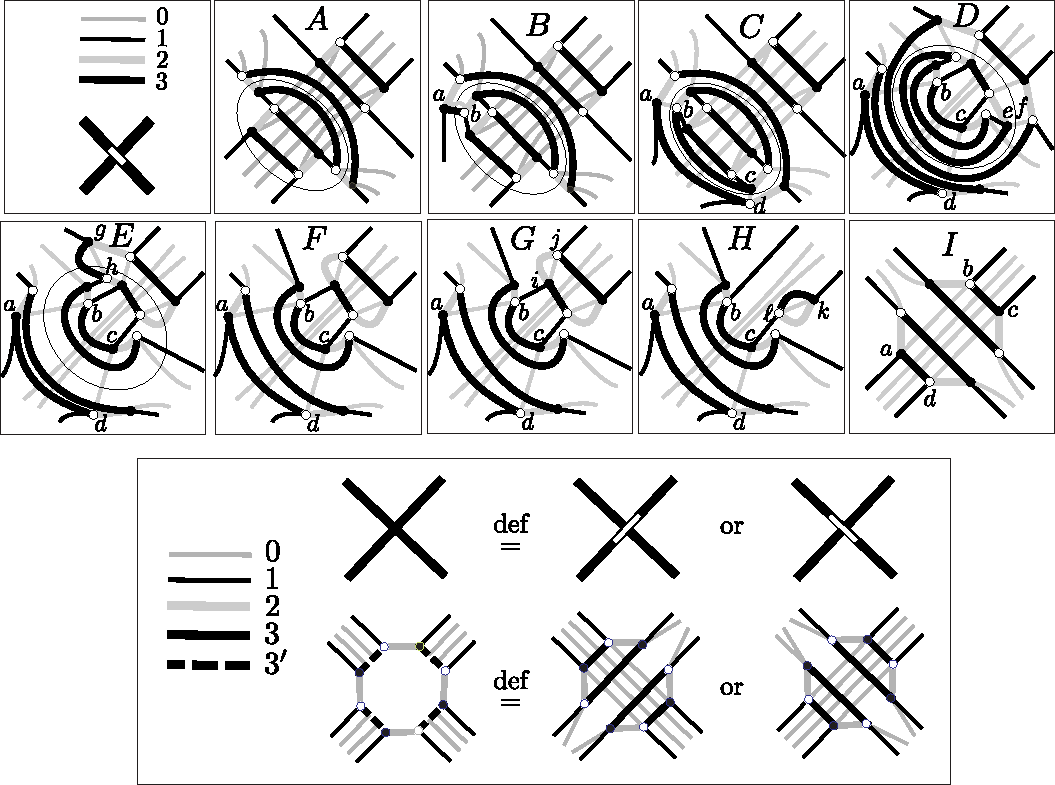
\includegraphics[width=15cm] {A.figs/12to8move.pdf}
\caption{\sf The $(12\to 8)$-simplification and the 
BFL $\to$ gem algorithm. 
}
\label{fig:12to8move}
\end{center}
\end{figure} 

In our context, a very important property of gems is that, given any
blackboard framed link with $n$ crossings there is an algorithhm to 
present a gem having $8n$ vertices which induce the same 3-manifold.
This algorithm is displayed at the bottom part of Fig. \ref{fig:12to8move}.
This was proved originally in Kauffman-Lins monography, page 175 of 
\cite{kauffman1994tlr},
which provide a gem with $12n$ vertices. By using an specific $TS$-move of 
\cite{lins1995gca} a gem with $8n$ vertices is obtained, page 81 of \cite{lins2007blink}.
The $(12\to 8)$-simplification by means of dipoles is depicted 
the upper part of Fig. \ref{fig:12to8move}.

\begin{figure}[!h]
\begin{center}
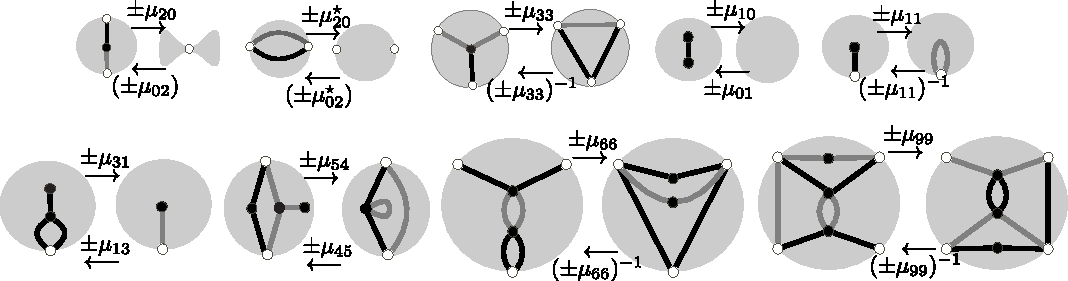
\includegraphics[width=15cm] {A.figs/reducedblinkcalculus.pdf}
\caption{\sf A (36-move,18-coin) reduced (sufficient) blink-coin calculus}
\label{fig:reducedblinkcalculus}
\end{center}
\end{figure}     

\subsection{A surprising new 1-1 correspondence and an $O(n^2)$-algorithm}
\label{subsec:surprise}

The present work is completely independent of Fig. \ref{fig:reducedblinkcalculus} 
and on the Theorems and on the Conjecture \ref{theo:incredible}, \ref{theo:O2algo}, 
\ref{theo:framedlink}, \ref{conj:remain} of this subsection, its reading
can be skipped at no logical cost. But we recommend the reader not to do so,
because the results and the Conjecture are stated to give a glympse and to clarify
our research in a broader appropriate context and timing.

Any closed, oriented 3-manifold is induced by some blink. Even though this object
has been around since 1994 when it was introduced in the joint research monography of L. Kauffman and
S. Lins, \cite{kauffman1994tlr}, the fact that they encode oriented closed 3-manifolds remains basically unkown.
This is about to change because as a consequence, \cite{lins2013B}, of a recent
result of B. Martelli, \cite {martelli2011finite,martelli2012finite}, each such a 
3-manifold becomes a subtle equivalence class of blinks.
In \cite{lins2013B}, a new calculus, this time on blinks, 
named {\em the blink-coin calculus} with 
8 types of local moves each applied to 8 types of related sub-blinks (named coins) are shown 
to capture the essence of homeomorphism between 3-manifolds, in the sense of 
Theorem \ref{theo:incredible}. A sufficent reduced blink-coin calculus with 36 moves is shown
in Fig. \ref{fig:reducedblinkcalculus}.
\begin{theorem}
\label{theo:incredible} 
Closed orientable 3-manifolds up to homeomorphism are blinks up to the blink-coin calculus.
\end{theorem}
The meaning of the theorem is that there exists a bijection 
$$\beta: \ \ \frac{{3\hspace{-1mm}-\hspace{-1mm}manifolds}}{{homeomorphisms}}\ \  
\longrightarrow\ \ \  \ \frac{blinks}{blink\hspace{-1mm}-\hspace{-1mm}coin \ calculus}.$$
If the manifold is given by a framed link, $\beta$ is obtained by a linear algorithm.
However, if it is given by a gem, by a triangulation, by a special spine 
\cite{matveev2007algorithmic},  
or by a Heegaard diagram, then a
polynomial algorithm to find $\beta$ seems to be an open problem. However, 
rescuing the situation there exists a recent work of S. Lins and his former student
R. Machado, which is reported in a sequence of 3-papers posted in the arXiv 
proving that there exists an 
$O(n^2)$-algorithm to go from a {\em resoluble} gem to a blink inducing the same 3-manifold.
\begin{theorem}
\label{theo:O2algo}
There exists an $O(n^ 2)$-algorithm to go from a {\em resoluble} gem to 
a blink inducing the same 3-manifold.
\end{theorem}
The parts of the work are available at 
\cite{linsmachadoA2012,linsmachadoB2012,linsmachadoC2012}. Even though 
the work leading to the above theorem is still being polished, 
we feel that is important to mention it here because they imply that there is
an $O(n^2)$-algorithm to find $\beta$ in the cases that the 3-manifold is given by a
resoluble gem. The proper definition of resoluble gem is still unecessary complicated
in the posted papers. Recently, in a still unpublished work, with the adequate definition 
of resolubility the same authors have proved the following theorem:
\begin{theorem}
\label{theo:framedlink}
If a 3-manifold is given by a framed link then there exists a linear algorithm
to obtain a resoluble gem inducing the same manifold.
\end{theorem}

Two gems induce the same 3-manifold if and only if they are linked by a finite
sequence of {\em blobs moves} and {\em valid flip moves}. This result is proved
for gems of arbitrary dimensions by S. Lins and M. Mulazzani in \cite{lins2006blobs}.
A {\em flip in a gem} is the recoupling of two equaly colored edges so as to maintain 
the bipartiteness. Flips that transform the $I$-dipole $\{u,v\}$ into the 
the $I \cup \{j\}$-dipole ($j \notin I \subset \{0,1,2,3\}$) and their inverses
are named {\em valid flips}. What is needed to close by polynomial algorithms 
between connecting these objects is to establish the following 
Conjecture which we feel is impossible to be false:

\begin{conjecture}
\label{conj:remain}
 A resoluble gem remains so under a blob move, or a valid flip move.
\end{conjecture}

If is true, as we are sure it is, the Conjecture means that there is an 
$O(n^ 2)$-algorithm to produce a blink inducing the same space as the one
given by an arbitrary gem, an arbitrary triangulation, an arbitrary
Heegaard diagram or an arbitrary special spine. Note that, as a bonus
we gain the capability of computing the Witten-Reshetikhin-Turaev invariants
\cite{reshetikhin1991invariants, kauffman1994tlr}
from the latter 4 presentations, what is currently impossible, because the 
WRT-invariants are only computable from blinks.

We stress that many interesting and deep consequences 
of Theorem \ref{theo:incredible} 
to the topology of 3-manifolds and to the combinatorics 
of plane graphs ought to exist.

 \subsection{Blackboard framed links}
 The pictures and the definitions  of this subsection are reproduced 
 from Section 12.1 of \cite{kauffman1994tlr}.
 It is included here for completeness since the concept is central in this work.
 Instead of working with the link in $\mathbb{R}^3$ it is to our 
 advantage to work with a {\em general position decorated projection} of the link
 into $\mathbb{R}^2$. Such projections are named {\em link diagrams}. 
 General position means that the pre-image of any
 point of $\mathbb{R}^2$ in the link is at most two points. A point that has
 two pre-image is a transversal crossing of two strands in the projection. Decorated means
 that we keep the information of which strand is the lower and which is the upper,
 usually by removing a small segment of the lower strand centered at the crossing.
 
 If $L$ is a link in $\mathbb{R}^3$ a {\em framed link based at $L$} is an embedding 
 $f: \mathbb{S}^1 \times [0,1] \longrightarrow \mathbb{R}^3$
 so that $L=f(\mathbb{S}^1 \times \{0\}).$ {\em Regular isotopy} is the class of
 link diagrams up to Reidemeister moves 2 and 3. Framed links are represented 
 by regular isotopy classes of link diagrams, with the extra move, 
 the {\em ribbon equivalence}, which
 is generated by the relations 
 \raisebox{-4mm}{
\includegraphics[width=6.7cm]{A.figs/ribbonrelation.pdf}} .
 
 With these extra relation, the ribbon equivalence classes of link diagrams 
 represent the framed links via the {\em blackboard framing}. This framing is 
 obtained by placing a vector field normal to each link component 
 with all the normals in the plane indicated by the diagram. We can indicate
 this this framing by sketching the tips of the normals as a second component,
 so that each component is indicated by an immersed band,
 see Fig. \ref{fig:doubledtrefoil}.
   
 \begin{figure}[!h]
\begin{center}
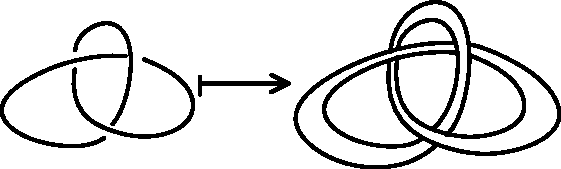
\includegraphics[width=11cm]{A.figs/doubledtrefoil.pdf} 
\caption{\sf How the tips of the normal vector field draws a second parallel component}
\label{fig:doubledtrefoil}
\end{center}
\end{figure} 
 
The reason for the ribbon equivalence is manifest in that the framings corresponding to these
two curls (with distinct winding number in the plane) are ambient isotopic:
$$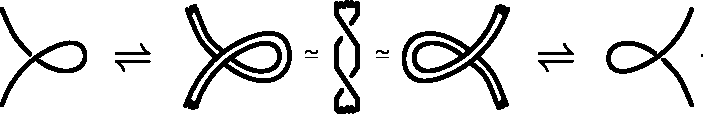
\includegraphics[width=11cm]{A.figs/ribbonmove.pdf}$$ 
We finish this subsection with a representative example of how to construct the 3-manifold
from the blackboard framed link. Suppose that the link diagram $K$ has just one component
and 3 curls corresponding to framing number 3 in $\mathbb{R}^3$:
$$
\includegraphics[width=4cm]{A.figs/linkL31.pdf}$$
Then $\mathbb{M}^3(K)$ is obtained by sewing $m \subset \mathbb{D}^2 \times \mathbb{S}^1$ to $\ell_K \subset
\mathbb{S}^3 \backslash (\mathbb{S}^1 \times \mathbb{D}^2)^{\tiny{o}},$ where $X^{\tiny{o}}$ means the 
interior of $X$. The sewing, forming the lens space $L_{3,1}$, is depicted below:
$$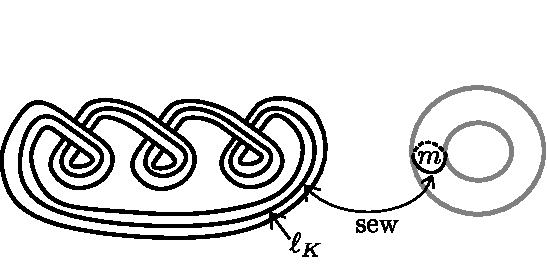
\includegraphics[width=10cm]{A.figs/generatingL31.pdf}.$$
Note that the longitudinal curve $\ell_K$ in the boundary of the
toroidal hole (which is identified with $m$ to close the toroidal hole)
never touches the boundary of the projection of 
the band formed by $K$ and its copy.

 
\subsection{The complementary roles of blinks and gems}

 Blinks are in 1-1 correspondence with blackboard framed links which in turn encodes every 
 closed oriented 3-manifold. If we consider these three 
 encodings of the same 3-manifold given in Fig. \ref{fig:blinklinkgem}, 
 the blink is the one that has the smallest ``perceptual complexity''. 
 The common manifold of this example is the binary tetrahedral space defined
 by $\mathbb{S}^3$ (as a topological continuos group) 
 up to the action of the non-comutative binary 
 tetrahedral group $\langle 3,3,2\rangle$, 
 (see \cite{magnus1966combinatorial}) which has 24 elements. The 3-manifold
 $\mathbb{S}^3/\langle 3,3,2\rangle$ has an spherical geometry. Its attractor
 (definition given shortly) consists
 of the single gem depicted at the right of Fig. \ref{fig:blinklinkgem}.

  
\begin{figure}[H]
\begin{center}
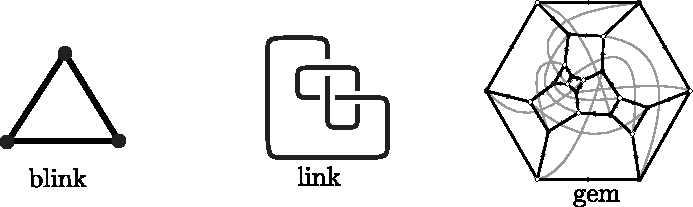
\includegraphics[width=11cm]{A.figs/blinklinkgem.pdf} 
\caption{\sf The minimum blink, minimum link and minimum gem inducing the 
binary tetrahedral space}
\label{fig:blinklinkgem}
\end{center}
\end{figure} 


 Blinks are very easy to generate recursively. They have a rich
 simpifying theory which permits the generation of 3-manifold catalogues. 
 Moreover, their isomorphism problem is computationally  simple. 
 Being blinks so good, why do we need gems? The 
 answer is that to prove that blinks induce the same 
 3-manifold (when they do) remains (probably even with the new blink-coin calculus)
 a very difficult problem. It is 
 straighforward to obtain a canonical gem from a blink, \cite{kauffman1994tlr,lins2007blink}.
 Proving that two gems induce the same
 3-manifold (when they do) is much easier because of the rich simplification 
 theory of them (based
 on at least 4 intertwined planarities) leading to the {\em attractors 
 of 3-manifolds}, \cite{lins1995gca}. These are defined as the set of gems inducing 
 the manifold having the minimum set of vertices. The important computational 
 point is that the attractor
 usually have few members, particularly if the manifold has a uniofolrm geometry
 euclidean, hyperbolic, spherical. 
 
  Blinks are very good at proving that two manifolds are distinct, because 
 from them we can extract
 the WRT-invariant, which is a very strong invariant, yet not a complete one. 
 These invariants currently 
 do not have a direct computation neither from triangulations, neither from gems,
 neither from Heegaard diagrams, neither from special spines of Matveev.
 In this respect see subsection \ref{subsec:surprise}, where we report progress
 on this issue.
 
 
 Gems and  blinks collaborate in a symbiotic dance to decide 
 (at a computational level) whether two 3-manifolds are or are not homeomorphic. 
 And many types of census  become available!  
 We present here our contribution to the topic.
 It is placed in the confluency of two deep passions of the authors:
 the study of closed orientable 3-manifolds and the study of plane 
 graphs. Here, we mean to provide a strategy for a 
 segmented answer of Hempel's questions posed at the introduction. 
 The closed oriented 3-manifolds are partitioned
 by the number of edges in a minimum encoding of them by a blink. 
  
 
Any plane drawing whatsoever of a graph with an arbitrary bipartition of its edge set, that is, a blink,
corresponds to a unique closed oriented 3-manifold via the associated 
blackboard framed links. An important aspect
about blinks is that each one possesses an easily obtainable {\em canonical form}
inducing the same 3-manifold: it is named the {\em representative of the blink} and is obtained
by lexicography from a small number of conventions, fixed in advance. 
This is explained, with a great amount of details, 
in L. Lins' thesis, \cite{lins2007blink}. 
\begin{figure}[H]
\begin{center}
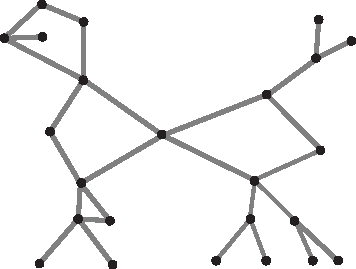
\includegraphics[width=6.5cm]{A.figs/doglikeblink.pdf} 
\raisebox{1.7cm}{
$\mapright{unique\  representative\ algorithm} {yielding\ the\ canonical \ form \ of \ the\ blink}$ }
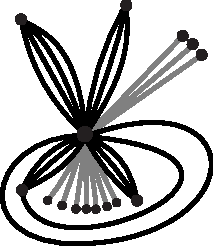
\includegraphics[width=3cm]{A.figs/repdoglikeblink.pdf} 
\caption{\sf Blink representative algorithm: doglike blink with 27 edges and its representative with 25 edges.}
\label{fig:doglikeblink}
\end{center}
\end{figure} 
 
 Lexicography is used to define a representative unique plane graph (a canonical form) 
 for each closed oriented 3-manifold. We explicitly solve the segmented problem 
 up to 9 edges, see Theorem \ref{theorem:census9}. This work provides 
 an efficient algorithm to make available the canonical form of any closed orientable 3-manifold
 induced by plane graphs at the current level of the catalogue (currently 9 edges) and, theoretically, this
 could be extended 10, 11,\ldots, $n$, for arbitrarily large $n$. Our theory gives a road to effectively
 name each 3-manifold classified by some set of invariants $INV$. We have a universal set of object, the blinks up
 to $n$ edges, which can be partitioned by these invariants. The $INV$-classes are then tried to be broken into
 homeomorphisms classes. New invariants are then discovered and added to $INV$ making them homeomorphisms classes 
 of $n$-small manifolds. The difficult cases are going to appear naturally and they lead to enhancement of
 the theory. It is not at all impossible that this process stops and we get $INV$ so 
 that the $INV$-classes be proved to  be homeomorphisms classes for all $n$. The point we want to make is that 
 good examples (hard to find, here exemplified by the $HG12QI$ classes 
 $9_{126}$ and $9_{199}$) are important in obtaining progress in a general theory.
 A classifying $INV$ for the 9-small 3-manifolds is
 $INV=\{{\ homology}, W\hspace{-0.5mm}RT_{12}, { \ length \ of\ smallest\  geodesic}\ \}.$

  

\section{Generating the $k$-universal set of blinks $U_k$}
\label{sec:generation}


A set of blinks is said to be $k$-universal if its members induce all $k$-small prime
3-manifolds. Note that the components of a blink is the same as the connected sum of 
the induced 3-manifolds. Therefore, our minimal sets of $k$-universal blinks are
composed of connected blinks. It is not difficult to implement an algorithm 
that produces a specific
$k$-universal set $U_k$. We start by (1) constructing all the 2-connected graphs having up to
$k$ edges, forming a set $A$. Then we take (2) all unions of blocks 
having a common vertex so that their edges 
set has at most $k$ edges. Regular isotopy shows that we can restrict to having all
blocks with a common vertex. Denote by $B$ the set of these combined blocks.
Next (3) we consider all bicolorations of the edges so that
the number of black edges is not smaller than the number of gray edges. We put the blink 
in the third set only if it coincides with its representative. This forms the set $C$.
Finally we use some topological filtering to decrease the size of $C$. The surviving blinks 
forms the set $D$, which is our $U_k$. A final comment we make about the generation is
that the connected blinks are implemented as embedded in $\mathbb{S}^2$. The external face
of a blink is well defined: namely is the face indexed with number 1 in the 
numbering which produces its code. At any rate, changing the external face
is easily done in the blink-coin calculus: it involve regular isotopy moves, 
one ribbon move and
one Whitney trick simplification.

\begin{figure}[H]
   \begin{center}
      \leavevmode
      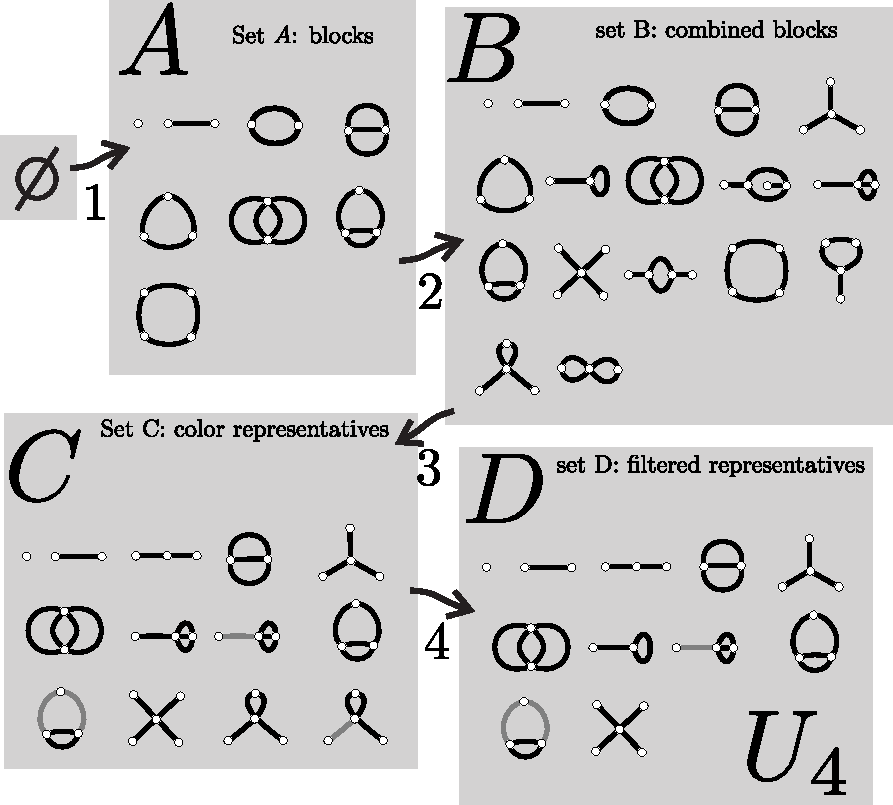
\includegraphics[width=11.5cm]{A.figs/4pipeline.pdf}
   \end{center}
   \vspace{-0.7cm}
   \caption{Pipeline for obtaining the set $U_k$ exemplified at $k=4$. Note that, starting
   with the empty set, the input of a phase is the output of the previous phase, that it,
   we have a pipeline. We must
   include the single vertex, as it corresponds to the unknot, inducing 
   $\mathbb{S}^2 \times \mathbb{S}^1$. The cardinality of $U_4$ is only 11.}
   \label{fig:4pipeline}
\end{figure}

The topological filters that we use are depicted in Fig. 
\ref{fig:SomeTopologicalFiltering}.
\begin{figure}[H]
\begin{center}
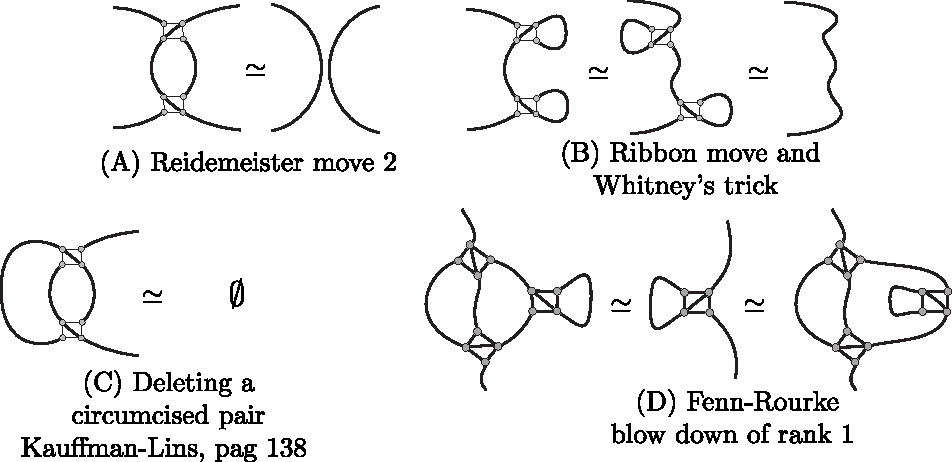
\includegraphics[width=11cm] {A.figs/SomeTopologicalFiltering.pdf}
\caption{\sf The topological filtering (at the level of blackborad framed links)
in the generation of $U_k$. BLINK has implemented
the pipeline generation of $U_9$ and $U_{10}$ with this filtering. 
They have respectively 3437 and 17948 blinks.
}
\label{fig:SomeTopologicalFiltering}
\end{center}
\end{figure}   

\section{Solving the 2 doubts left in L. Lins thesis}
\label{sec:resol}





\subsection{Unveiling the mistery of the two doubts}
The topological classification of the 9-small spaces was nearly completed in 
\cite{lins2007blink}. This work develops a theory for generating a distinguished
set of blinks named $U_n$ and indexed lexicographically, $U_n[i]$ is the $i$-th such blink.
This has been revewed
The relevance of $U_n$ is that it misses no closed, orientable, prime and irreducible
3-manifold which is induced by a blink up to $n$ edges. 

\begin{figure}[H]
\begin{center}
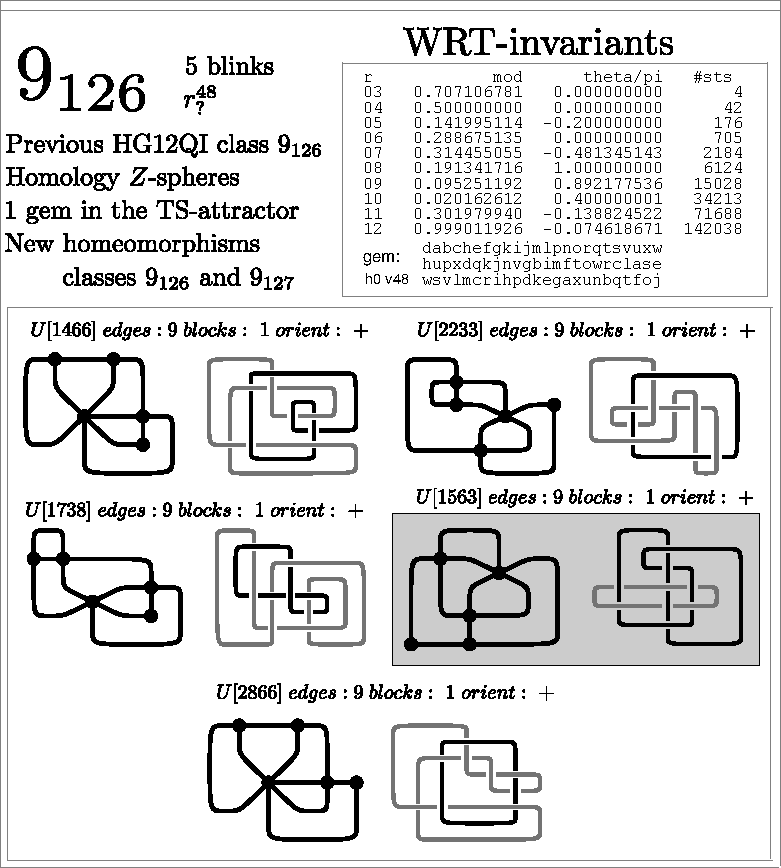
\includegraphics[width=8cm]{A.figs/nine126.pdf}
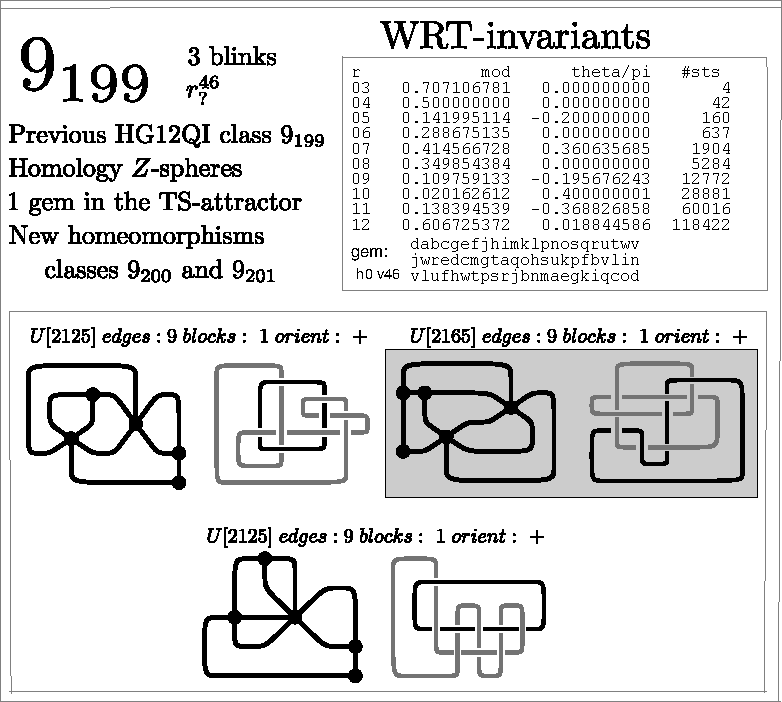
\includegraphics[width=8cm]{A.figs/nine199.pdf}
\caption{\sf The two doubts left in L. Lins's thesis are solved 
In both cases the manifolds induced
by the shaded blink-link pairs are proved very recently to be non-homeomorphic 
to the other in the same class, by geometric means. All the other pairs are proved 
to be homeomorphic by BLINK which keeps each such homeomorphism as a coded sequence which
is stored in a data basis, and, in principle reproducible at will. 
This shows that BLINK finds all available homeomorphic pairs and, in conjunction with
the length of the samllest geodesic (see next section), provides
the topological classification of the 9-small 3-manifolds.}
\label{fig:nine126nine199}
\end{center}
\end{figure} 

The 3-manifolds of \cite{lins2007blink} are classified by homology and the quantum WRT$_r$-invariants
$r=3,\ldots,u$, with $10$ significant decimal digits forming $HGuQI$-classes of blinks. 
Our algorithm for computing the 
$WRT_r^u$-invariants are based on the theory developed in \cite{kauffman1994tlr}.
After 6 years we have put our doubts as a Challenge to topologists and 
group algebraists, \cite{linslins2013A}. They were quickly solved by some researchers among others
M. Culler, N. Dunfield and C. Hodgson, at least in two different ways. They proved that the two pairs of
manifolds which were left unresolved by BLINK are indeed non-homeomorphic. All the other pairs
in the $HG12QI$-classes $9_{126}$ and $9_{199}$ have been checked to be homeomorphic, as BLINK proved
6 years ago. The new solutions were obtained using the software \cite{snappy}, which uses 
the kernel of \cite{weeks2001snappea}. They also use GAP (\cite{gap2002gap}) and Sage (\cite{sage2012}). 
 
The first solution is by C. Hodgson using length spectra techniques, based in his
joint paper with J. Weeks entitled {\em Symmetries, 
isometries and length spectra of closed hyperbolic three-manifolds} 
(\cite{hodgson1994symmetries}). By using SnapPy Hodgson showed that even though the 
quantum WRT-invariants as well as the volumes of the 
hyperbolic $Z$-homology spheres induced by the blinks
$U[1466]$ and $U[1563]$ are the same, the {\em length of the 
smallest geodesics of them are distinct}. As for the other pair of blinks, $U[2125]$ and $U[2165]$, 
the same facts apply. Here is a summary of Hodgson's findings extracted from the SnapPy session
that he kindly sent us. As he explains: {\em ``The output of the length spectrum 
command shows the {\em complex lengths}
of closed geodesics --- the real part is the actual length and the imaginary 
part is the rotation angle
as you go once around the geodesic.''}\\
\begin{center}
\center{Class $9_{126}$:}
\begin{verbatim}
First geodesic of U[1466]: 1.0152103824828331+0.39992347315914334i.
First geodesic of U[1563]: 0.9359206605025168+2.333526236965665i.
Volume of both manifolds: 7.36429600733.
\end{verbatim}
\center{Class $9_{199}$:}
\begin{verbatim}
First geodesic of U[2125]:  0.8939075859248593+0.761197185679321i.
First geodesic of U[2165]:  0.7978548001747316+2.9487425029345973i.
Volume of both manifolds: 7.12868652133.
\end{verbatim}
\end{center}


\section{Conclusion}
A closed orientable 3-manifold is denoted {\em $n$-small} if it is induced by surgery on
a blackboard framed link with at most $n$ crossings. We provide an instance of the general theory
to produce a recursive indexation of $n$-small 3-manifolds up to homeomorphism. We 
solve this problem
up to $n=9$. Conceptually we could go on forever, finding in the way 
tougher and tougher examples to be distinguished
by yet to be found new invariants.
 The topological classification of the 9-small 3-manifolds involve three invariants: 
 $$INV=\{{\ homology}, \ W\hspace{-0.5mm}RT_{12}, { \ length \ of\ smallest\  geodesic}\ \}.$$
 The classification was nearly complete in \cite{lins2007blink}, except for two doubts. Recently,
 after we posted a challenge in the arXiv, \cite{linslins2013A} these doubts were solved by
 M. Culler, N. Dunfield and C. Hodgson using SnapPy \cite{snappy}. This made us add 
 $$ \ length \ of\ smallest\  geodesic $$ 
 which we define as 0, if the manifold is not hyperbolic, to our list of invariants. 
 The $9$-small 3-manifold classification maintains live the two Conjectures 
 of page 15 of \cite{lins1995gca} based on two kinds of moves $TS$ and $U$:
 the $TS$- and $U$-moves yield an efficient algorithm to classify 3-manifolds 
 by explicitly displaying homeomorphisms among them, whenever they exist. 
 A recent finding by C. Hodgson concerning manifolds $T[71]$ and $T[79]$ forming the 
 HG8QI-class $14_{24}^t$, in the notation of page 239 of \cite{lins2007blink} shows that 
 the 3 invariants are not enough to
 decide the pair. This pair is the first one of 11 pairs that we display as some tougher challenges
 to 3-manifold topologists, \cite{lins2013}. Hodgson's finding is that the volume as well as the
 lengths of the smallest geodesics fail to distinguish $T[71]$ and $T[79]$. He proves them 
 to be non-homeomorphic by more sofisticated techniques, involving drilling along the smallest geodesics
 to get non-isometric manifolds with toroidal boundary. Using SnapPy, GAP and Sage, 
 N. Dunfield shows that $T[71]$ and $T[79]$  are also distinguished by the homology of 
 its 5-covers. This solution depends on the existence of low index subgroups of the 
 fundamental group of the manifold. What about if they do not exist? We feel that
 the majority of the {\em Tough Challenges} of \cite{lins2013} remains unresolved.
 Have we arived to our currently technological limit? Maybe so, but what we feel the 
 difficulty of SnapPy and BLINK in dealing with the tough challenges teach us is
 that we need better subtle invariants computed quicky than the current ones. 
 Invariants which are not so exponential
 as looking for small index coverings which depend on the fundamental group. 
 The $HG8QI$-class $16_{42}$ is composed of 4 blinks 
 $\{T[305]$, $T[337]$, $T[387]$, $T[420]\}$, in the notation of 
 \cite{lins2007blink, lins2013}. BLINK says that there is at most 2 homeomorphic classes.
 We believe this bound is attained. However SnapPy computed the homology of 4-covers
 of these spaces and they all agree. We conjecture that there is an invariant which
 breaks the $HG8QI$-class $16_{42}$ into two homeomorphic classes of two blinks each. 
 We finish this paper with a focused challenge: prove or disprove this conjecture.
 The relevant blackboard framed links are shown in Fig. \ref{fig:T16_42focusedchallenge}
 
\begin{figure}[H]
\begin{center}
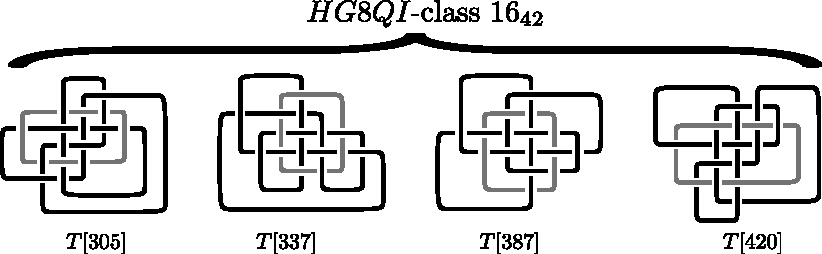
\includegraphics[width=14cm] {A.figs/T16_42focusedchallenge.pdf}
\caption{\sf The $HG8QI$-class $16_{42}$. We conjecture that 
there are exactly two homeomorphism classes induced by these 4 blackboard framed links
in $16_{42}$, and that each class is induced by 2 of the BFL's above.
BLINK tell us that there is at most 2 homeomorphism classes,
(each induced by two blinks) and SnapPy/Sge/GAP 
showed that the 4 blinks induced 3-manifold have 4-coverings with the same homology
(tests effected by C. Nascimento). Coverings of other indices have been very slow
to compute. We do not know whether SnapPy can get isomophic
triangulation for the 4 blinks. We bet not, BLINK would have found them. Asssuming
that there are two homeomorphism classes, which computable invariant will distinguish
them? Have we reached our current technological limit with this example? 
If so, we need badly to discover new invariants.
The eleven examples (of which $HG8QI$-class $16_{42}$ is the fifth) 
forming the touger challenges in $\cite{lins2013}$ must be taken seriously.
To us most of them remain open. It seems that if they can be solved at all, it will
be by luck, involving very expensive computations. We need
something better.
}
\label{fig:T16_42focusedchallenge}
\end{center}
\end{figure} 
 

 
 
%-----------------------------------
\bibliographystyle{plain}
%\bibliographystyle{is-alpha}
%\addcontentsline{toc}{bibliografia}{\MakeTextUppercase{Refer�ncias Bibliogr�ficas}}
%\bibliography{d:/slsl\3.DadosSostenes.35.ArtigosLivros.bibtexGoogleScholar/bibtexIndex.bib} % bib file is slsl.bib
%\bibliography{~/home/ricardo/Dropbox/35.ArtigosLivros.bibtexGoogleScholar/bibtexIndex.bib}
\bibliography{bibtexIndex.bib}
%\bibliography{slsl}


\vspace{5mm}
\begin{center}
\hspace{7mm}
\begin{tabular}{l}
   S\'ostenes L. Lins\\
   Centro de Inform\'atica, UFPE \\
   Av. Jornalista Anibal Fernandes s/n\\
   Recife, PE 50740-560 \\
   Brazil\\
   sostenes@cin.ufpe.br
\end{tabular}
\hspace{20mm}
\hspace{7mm}
\begin{tabular}{l}
Lauro D. Lins\\
AT\&T Labs Research \\
180 Park Avenue \\
Florham Park, NJ 07932 \\
USA\\
llins@research.att.com
\end{tabular}
\hspace{20mm}

\end{center}

\newpage
\section{Appendix: census (no misses, no duplicates) of 9-small 3-manifolds}
\subsection*{Part 1/4 in terms of blinks:}
\center{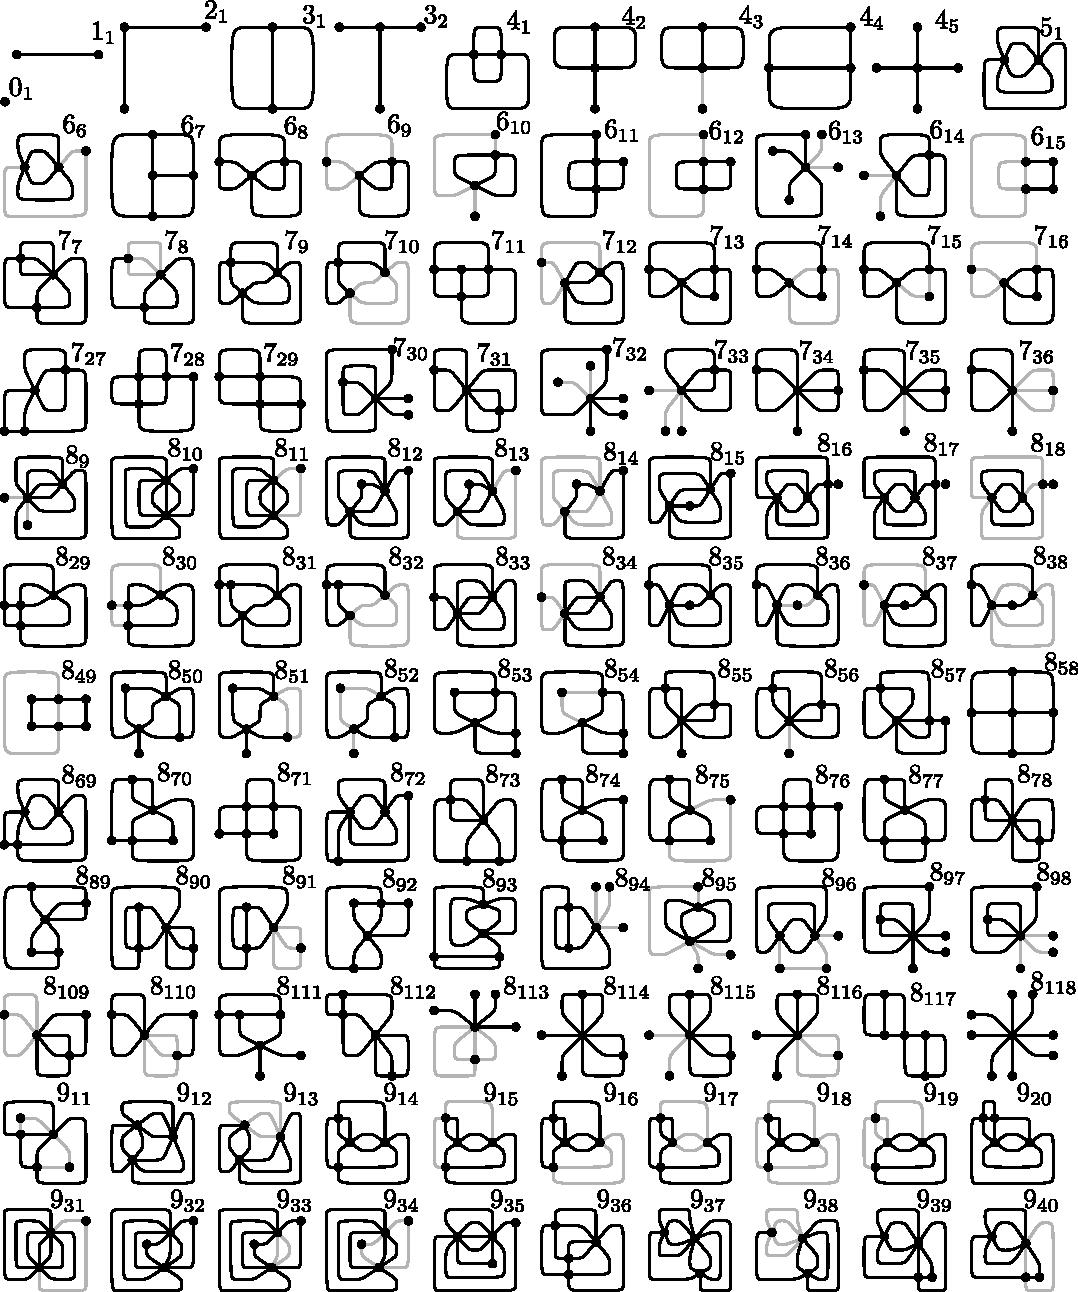
\includegraphics[width=16.5cm]{A.figs/primes489m11.pdf}} \eject \noindent
\subsection*{Part 1/4 in terms of blackboard framed links:}
\center{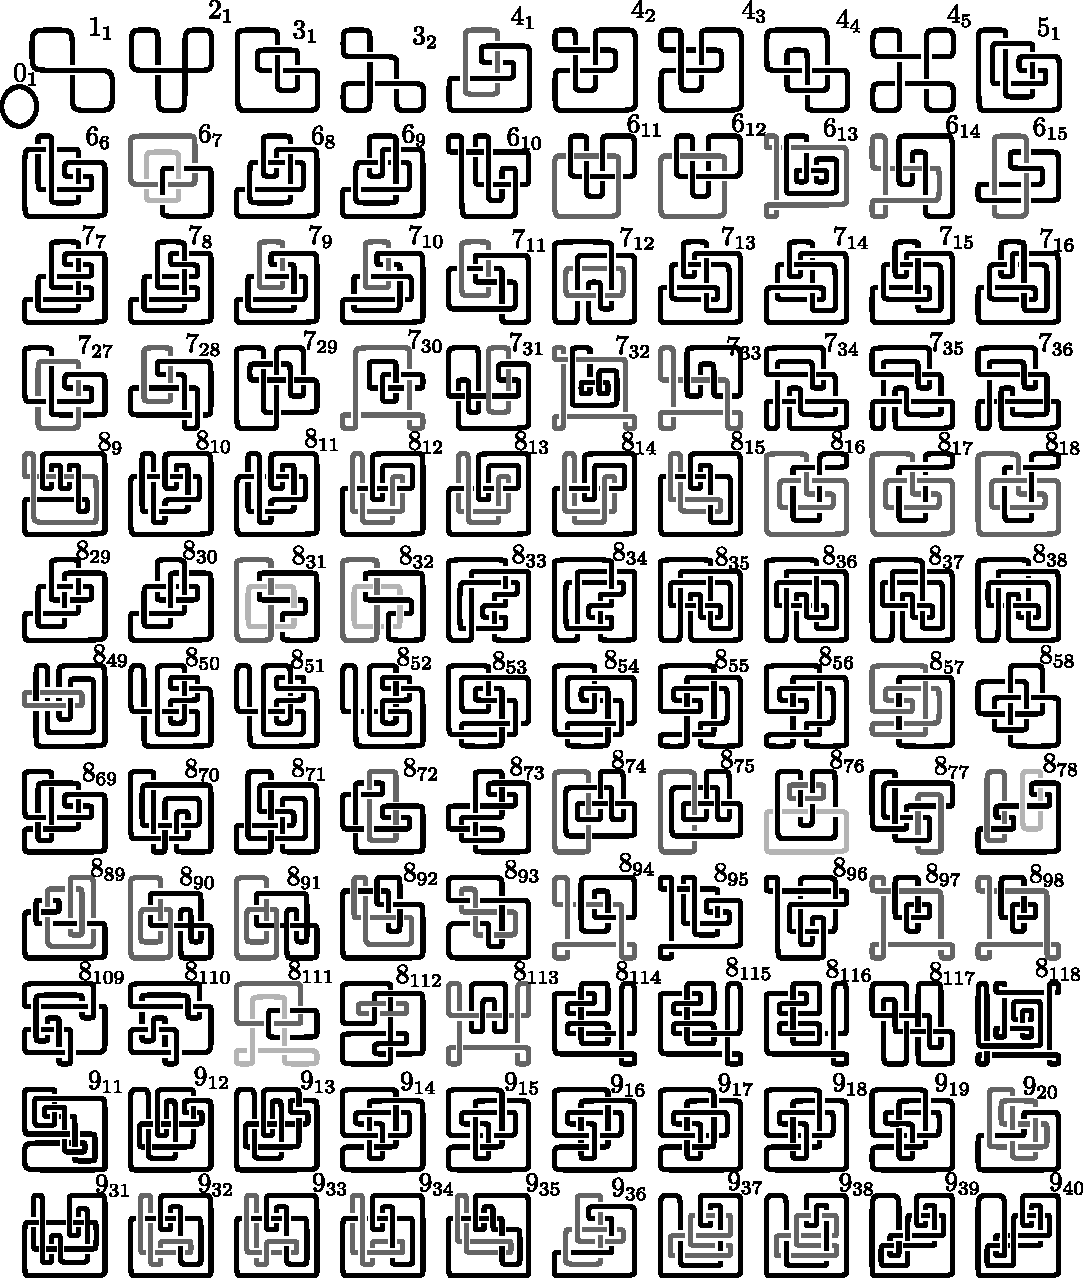
\includegraphics[width=16.5cm]{A.figs/primes489linksm11.pdf}} \eject
\subsection*{Part 2/4 in terms of blinks:}
\center{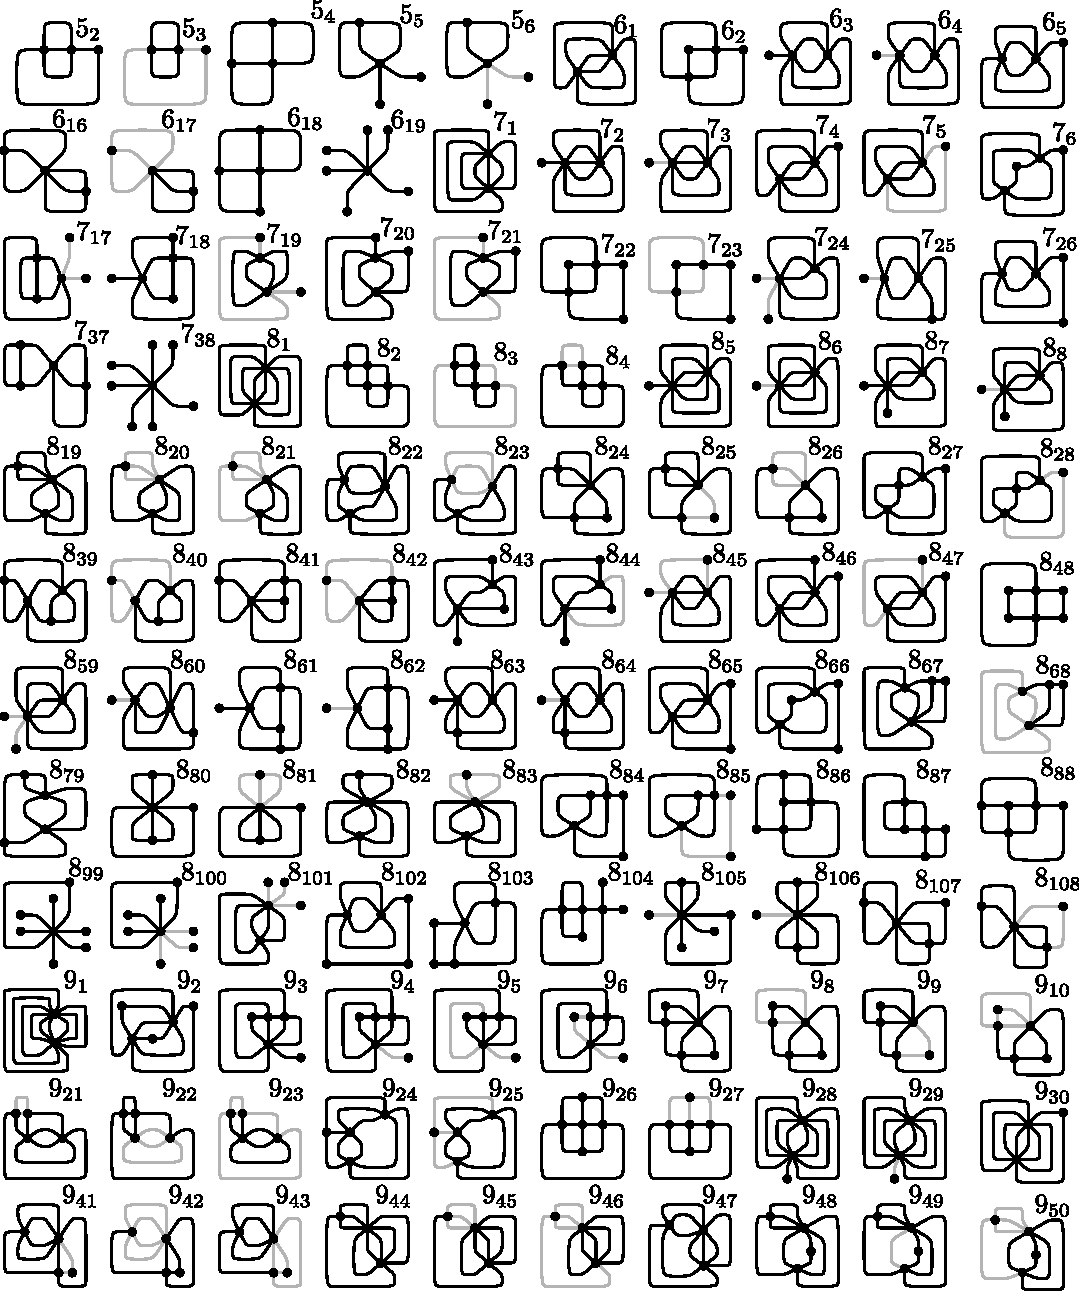
\includegraphics[width=16.5cm]{A.figs/primes489m12.pdf}} \eject
\subsection*{Part 2/4 in terms of blackboard framed links:}
\center{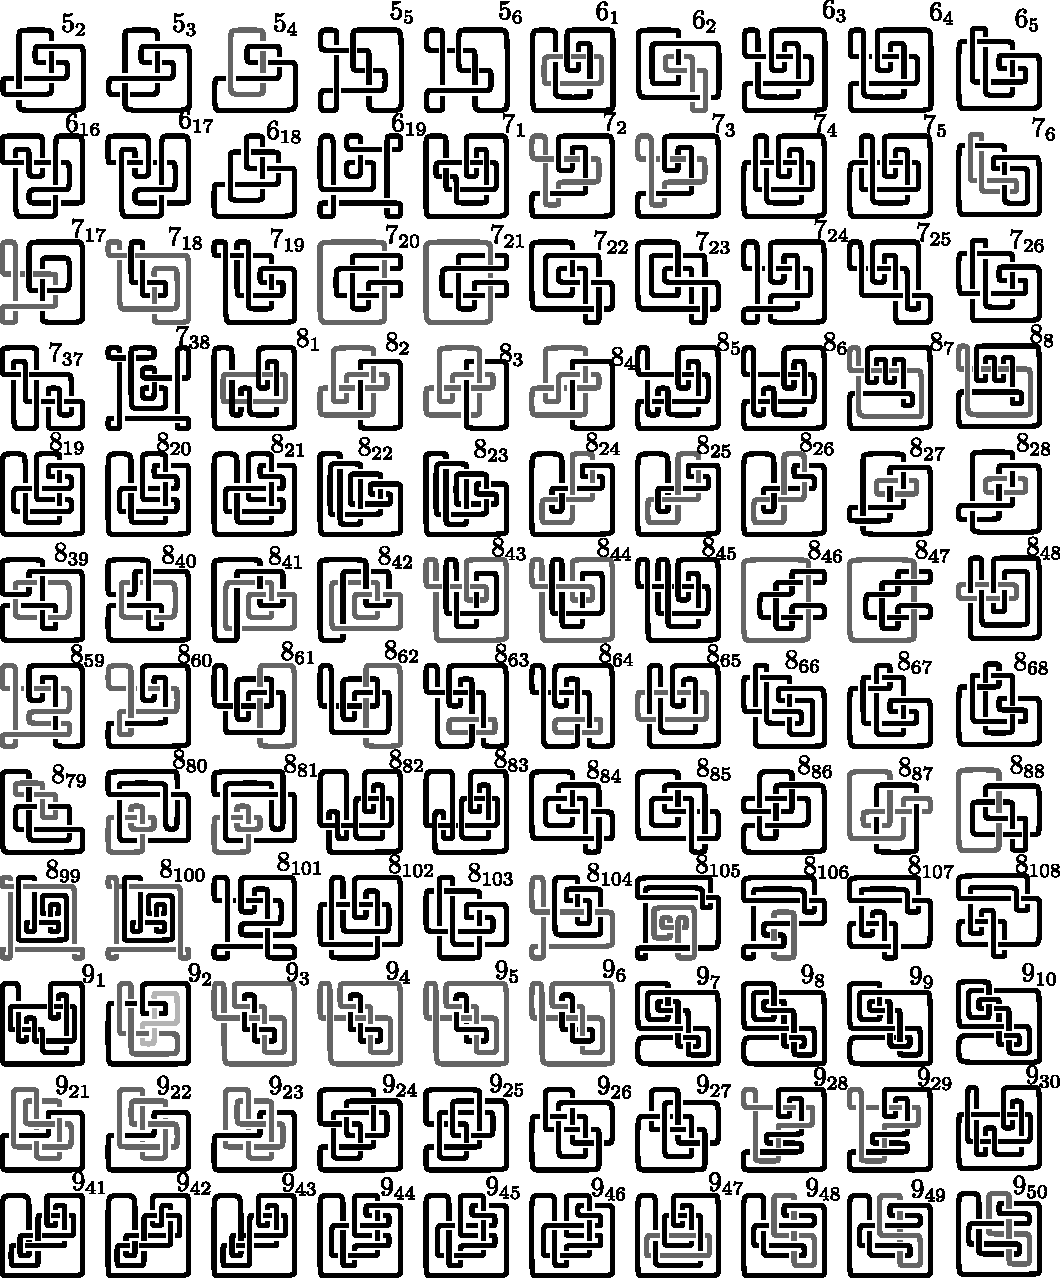
\includegraphics[width=16.5cm]{A.figs/primes489linksm12.pdf}} \eject
\subsection*{Part 3/4 in terms of blinks:}
\center{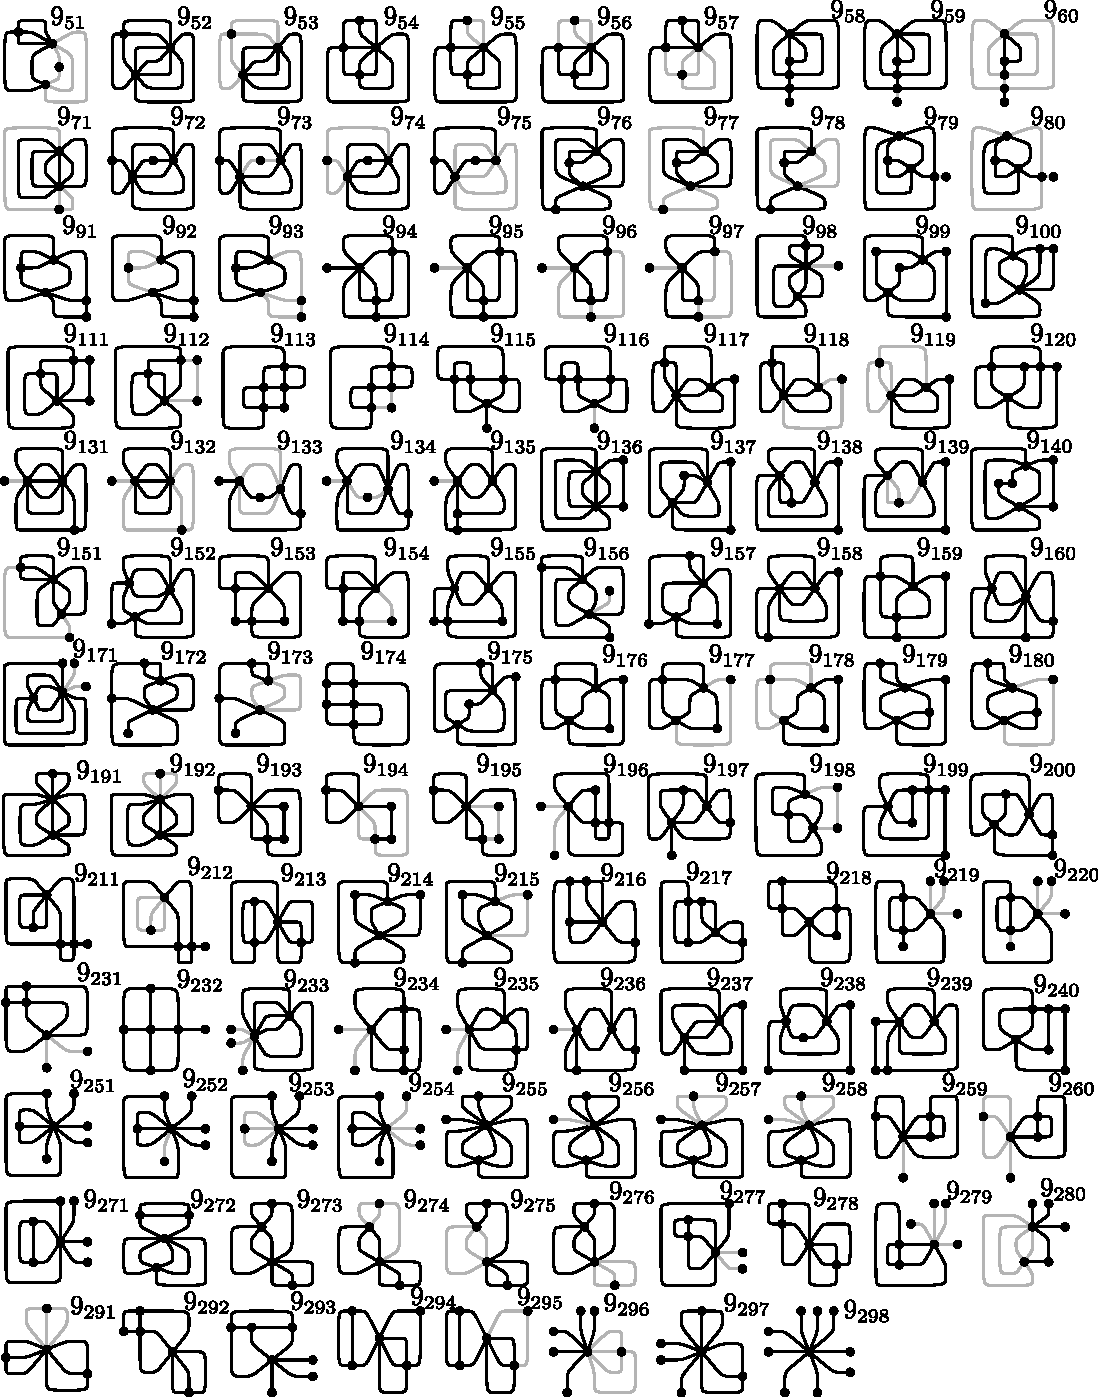
\includegraphics[width=16.5cm]{A.figs/primes489m21.pdf}} \eject
\subsection*{Part 3/4 in terms of blackboard framed links:}
\center{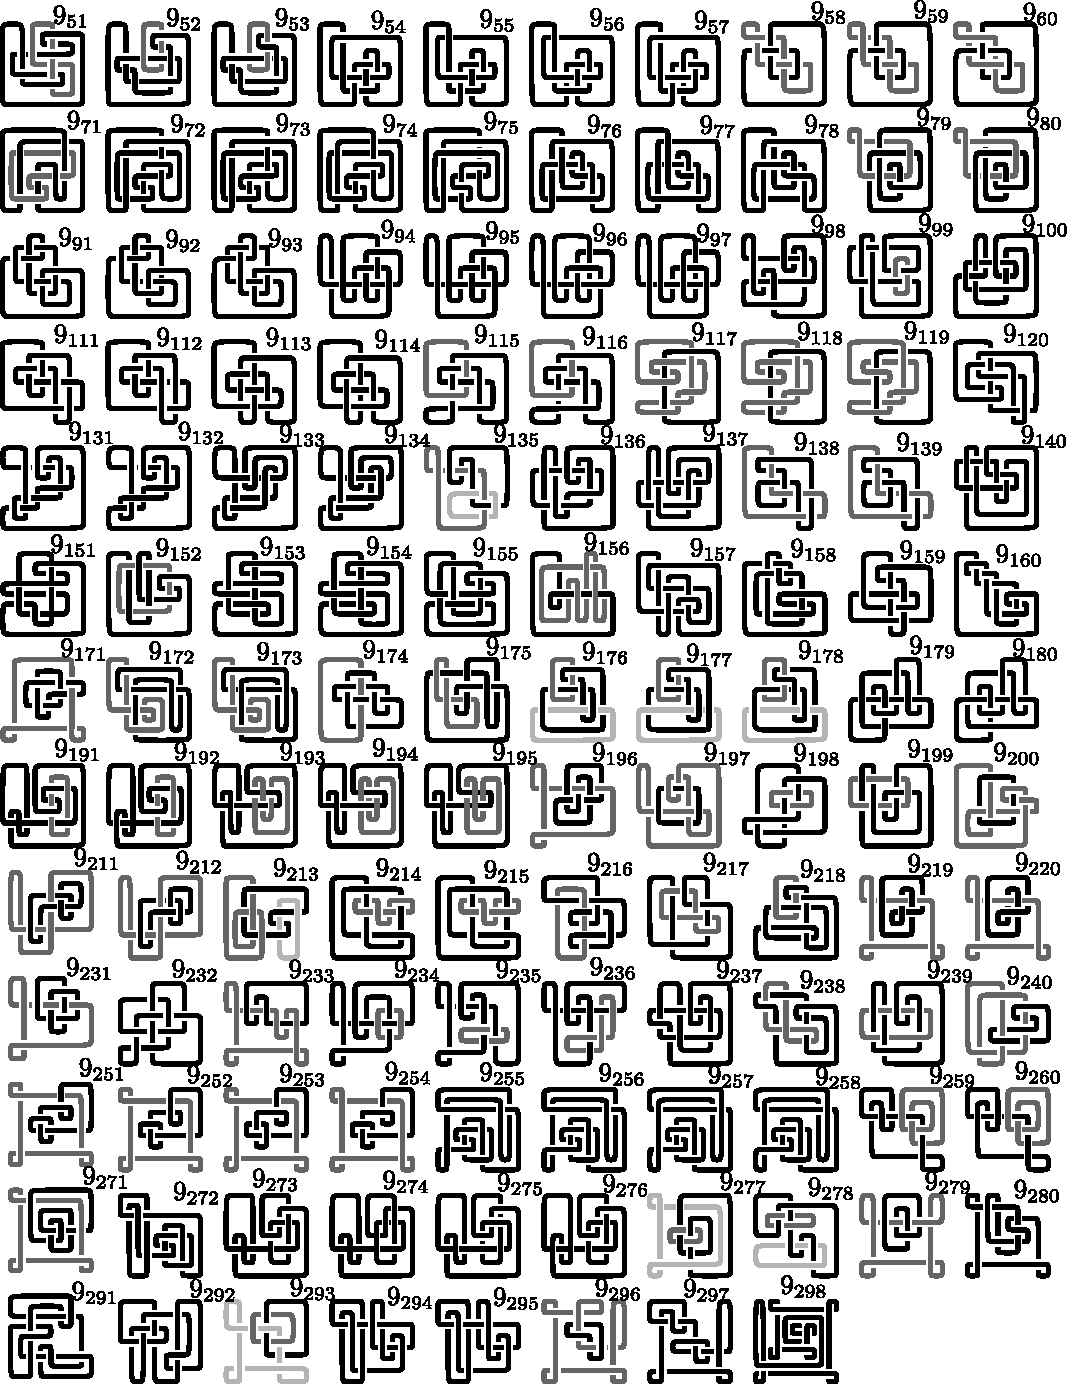
\includegraphics[width=16.5cm]{A.figs/primes489linksm21.pdf}} \eject
\subsection*{Part 4/4 in terms of blinks:}
\center{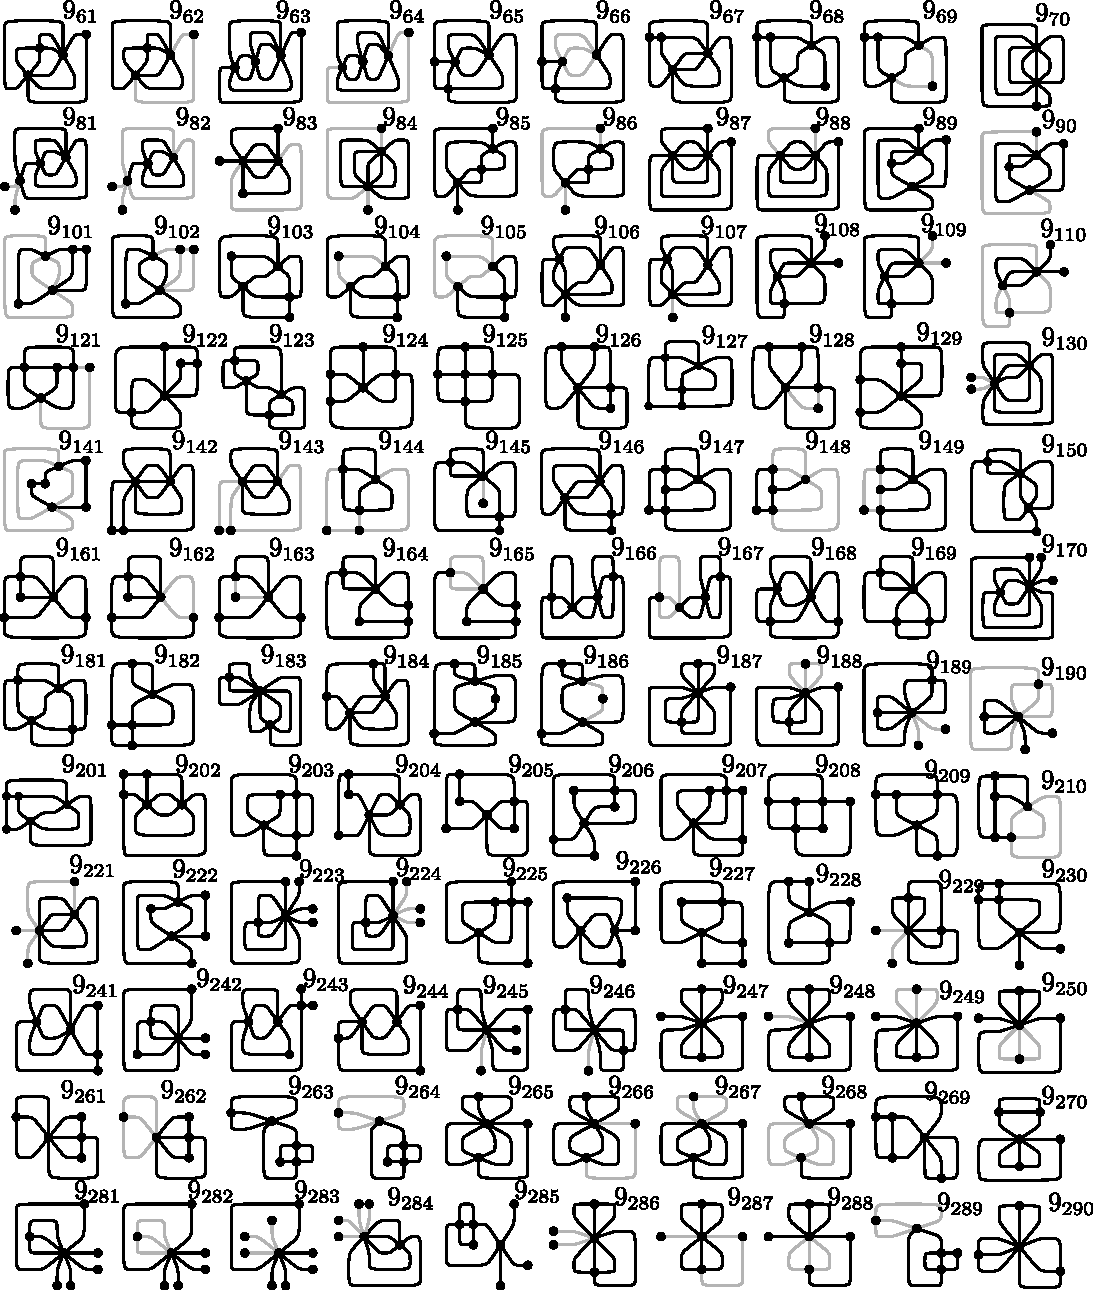
\includegraphics[width=16.5cm]{A.figs/primes489m22.pdf}} \eject
\subsection*{Part 4/4 in terms of blackboard framed links:}
\center{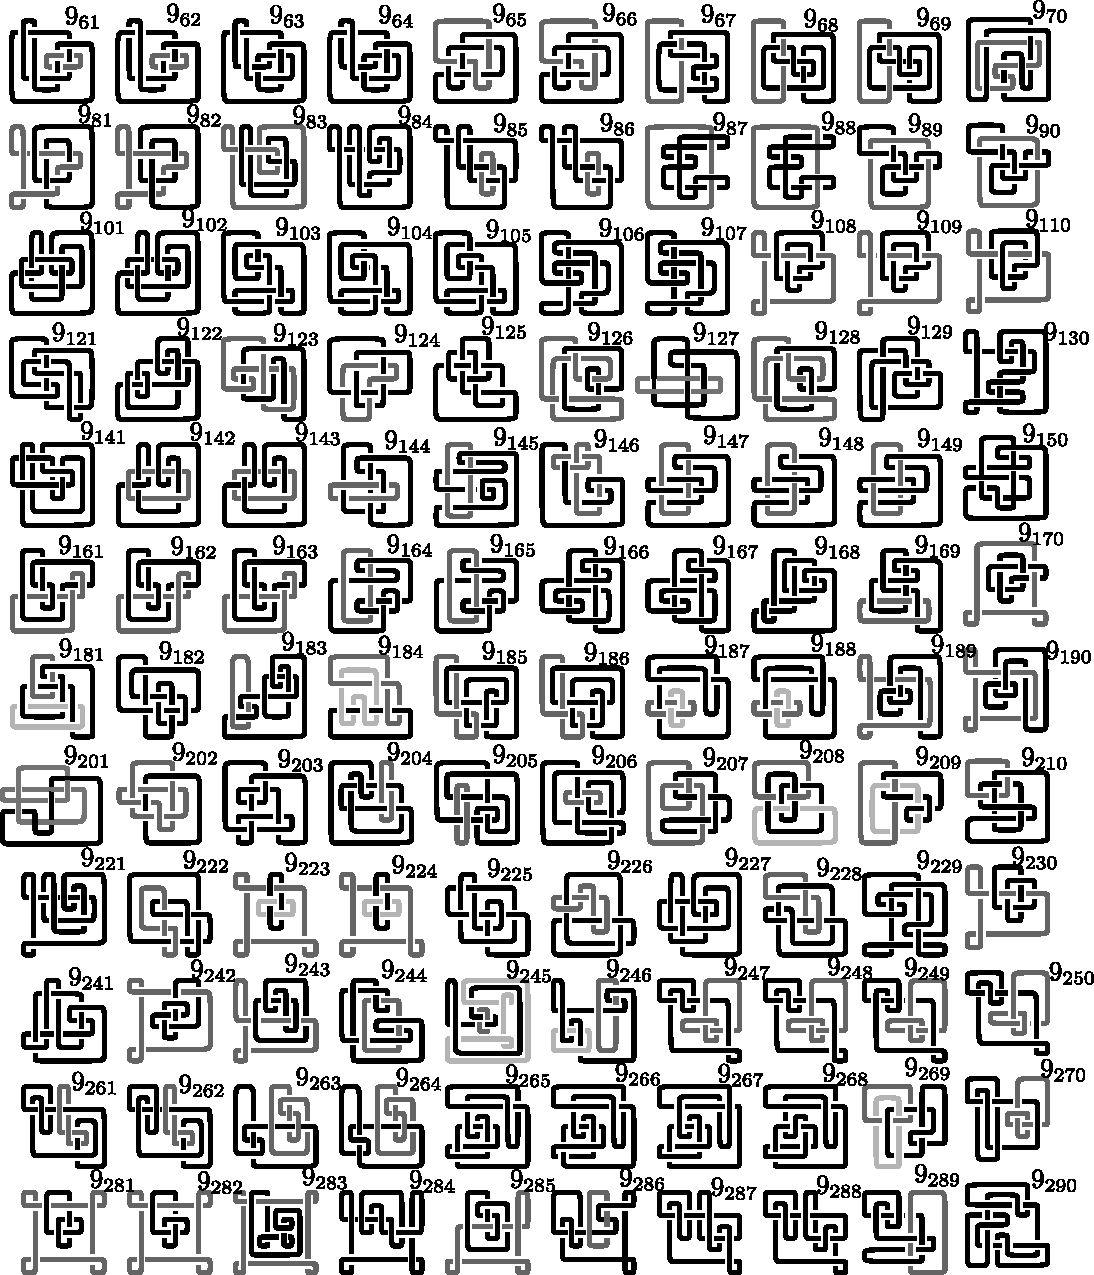
\includegraphics[width=16.5cm]{A.figs/primes489linksm22.pdf}}\eject





\end{document}


% \printindex
